\documentclass[fullpage,a4paper]{article}

\usepackage{amsmath}
\usepackage{amssymb}
\usepackage{amsthm}
\usepackage{bm}
\usepackage{authblk}
\usepackage{graphicx}
\usepackage{csquotes}
\usepackage{todonotes}
\usepackage{listings}
\usepackage{url}

\renewcommand{\v}[1]{\bm{#1}}
\newcommand{\vx}{\v{x}}
\newcommand{\vt}{\v{\theta}}
\newcommand{\vb}{\v{\beta}}
\newcommand{\vm}{\v{m}}
\newcommand{\R}{\mathbb{R}}
\newcommand{\E}{\mathbb{E}}
\newcommand{\Var}{\mathbb{V}ar}
\renewcommand{\P}{\mathbb{P}}
\newcommand{\Q}{\mathbb{Q}}
\newcommand{\D}{\mathcal{D}}

\newcommand{\eq}[1]{Eq.~(\ref{eq:#1})}
\newcommand{\fig}[1]{Fig.~\ref{fig:#1}}
\newcommand{\hyp}[1]{Hyp.~\ref{hyp:#1}}

\newtheorem{definition}{Definition}
\newtheorem{hypothesis}{Hypothesis}
\newtheorem{theorem}{Theorem}

\title{A visual explanation of country specific differences in
  Covid-19 data.}
\author{Nils Bertschinger}

\begin{document}

\maketitle%%

\begin{abstract}
  This report provides a visual examination of Covid-19 case and death
  data. In particular, it shows that country specific differences can
  too a large extend be explained by two easily interpreted
  parameters. Namely, the delay between reported cases and deaths and
  the fraction of unoberved cases. Furthermore, this allows to lower
  bound the actual total number of people already infected.
\end{abstract}

\section{Introduction}

The world stands still ... desperately observing the unfolding of the
global COVID-19 pandemic.

\section{Data exploration}

Covid-19 data are published by several sources, most notably the John
Hopkins university and the European Center for Decease Prevention and
Control (ECDC). Here, data from ECDC as available from
\url{https://opendata.ecdc.europa.eu/covid19/casedistribution/csv} are
used.

\begin{figure}
  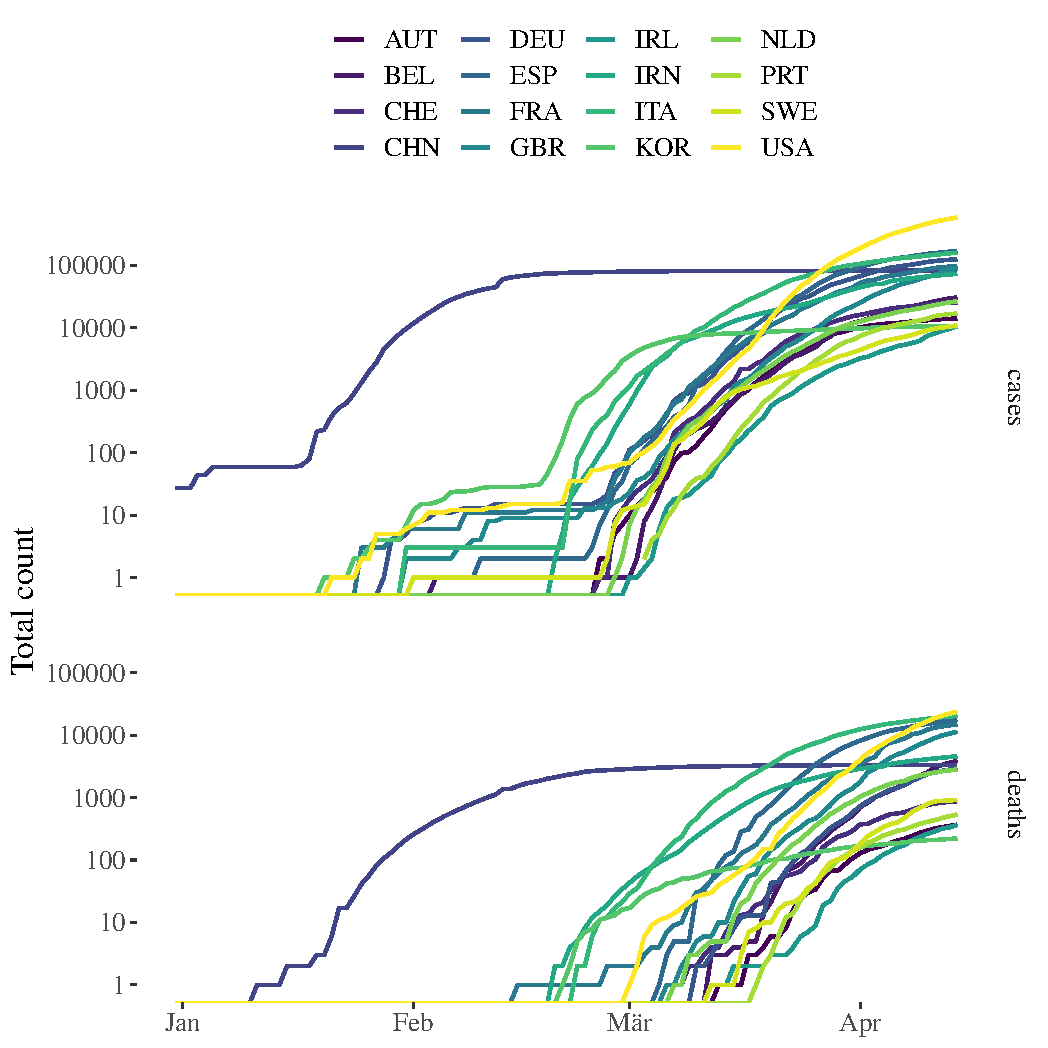
\includegraphics[width=0.495\textwidth]{../figs/ecdc_raw_absolute.pdf}
  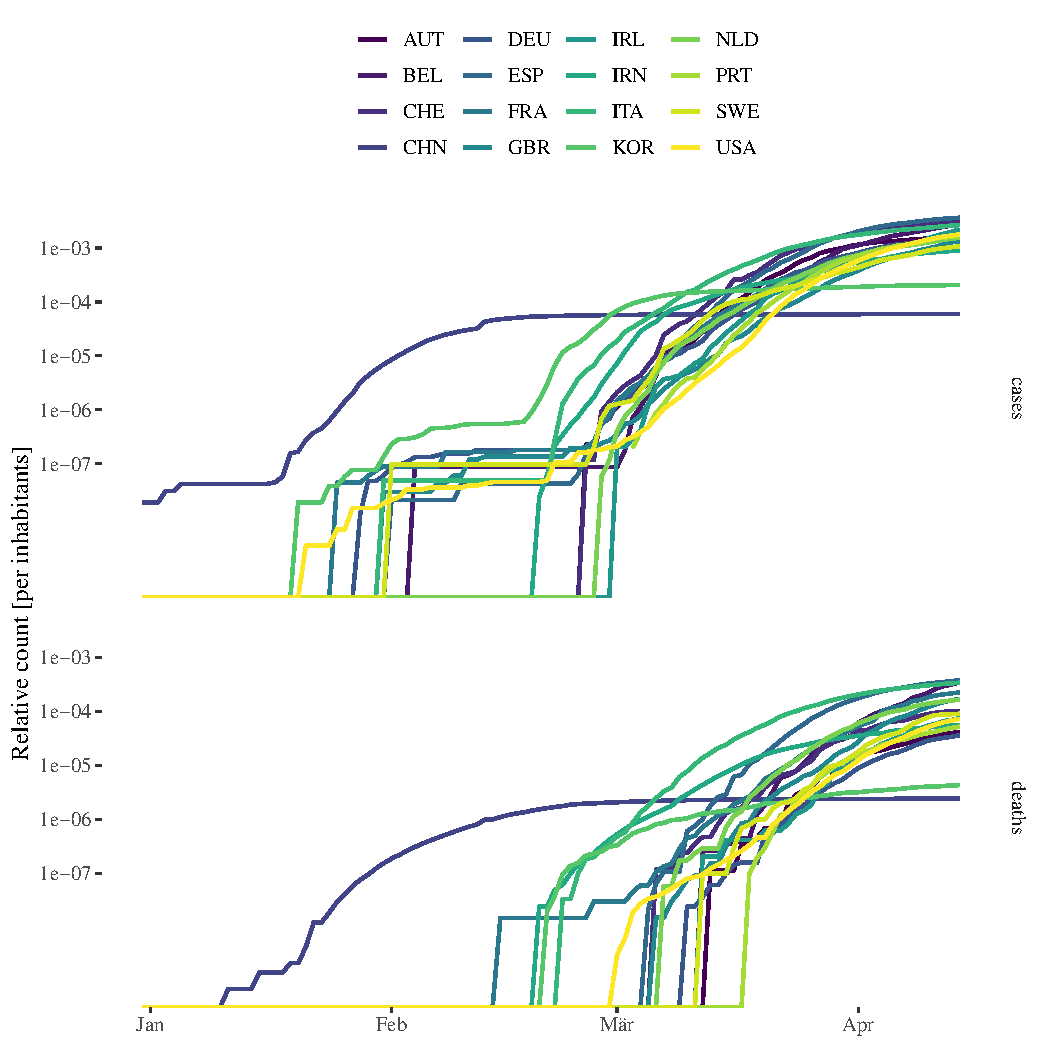
\includegraphics[width=0.495\textwidth]{../figs/ecdc_raw_relative.pdf}
  \caption{\label{fig:raw_data} Case and death counts of selected
    countries. Both in absolute (left) and relative (right), i.e. per
    inhabitants, terms.}
\end{figure}
\fig{raw_data} shows the total cumulative case and death counts of
selected countries. These countries are among the eight most effected
countries in terms of absolute and relative deaths\footnote{In
  addition, South Korea is included as its numbers are commonly
  considered of high quality.}. In the following, I will focus on
relative counts as these are arguably more meaningful when comparing
different countries -- which could differ widely in terms of
population size.

\begin{hypothesis}
  \label{hyp:count}
  Death counts are more reliable than case counts.
\end{hypothesis}

By \hyp{count} analysis will start from relative cumulative death
counts $d_t$ in the following\footnote{Similarly, relative cumulative
  case counts are denoted as $c_t$}. Furthermore, in order to
facilitate country comparisons, dates are shifted relative to the
first day that relative death counts exceed a threshold $\theta$ of
$1, 2, 4$ or $8$ deaths per million inhabitants respectively, i.e. $t
= 0$ is defined such that $d_t \geq \theta$ for $t \geq 0$ and $d_t <
\theta$ for $t < 0$. \fig{aligned_data} shows the resulting time
course of relative case and death counts. Aligning dates in this
fashion shows that several countries exhibit similar time courses,
e.g. Belgium and Spain or China and South Korea. Yet, there are
unexplained country specific differences and the data collapse is not
as convincing as often observed in physical systems exhibiting scaling
laws \cite{stanley99}.
\begin{figure}
  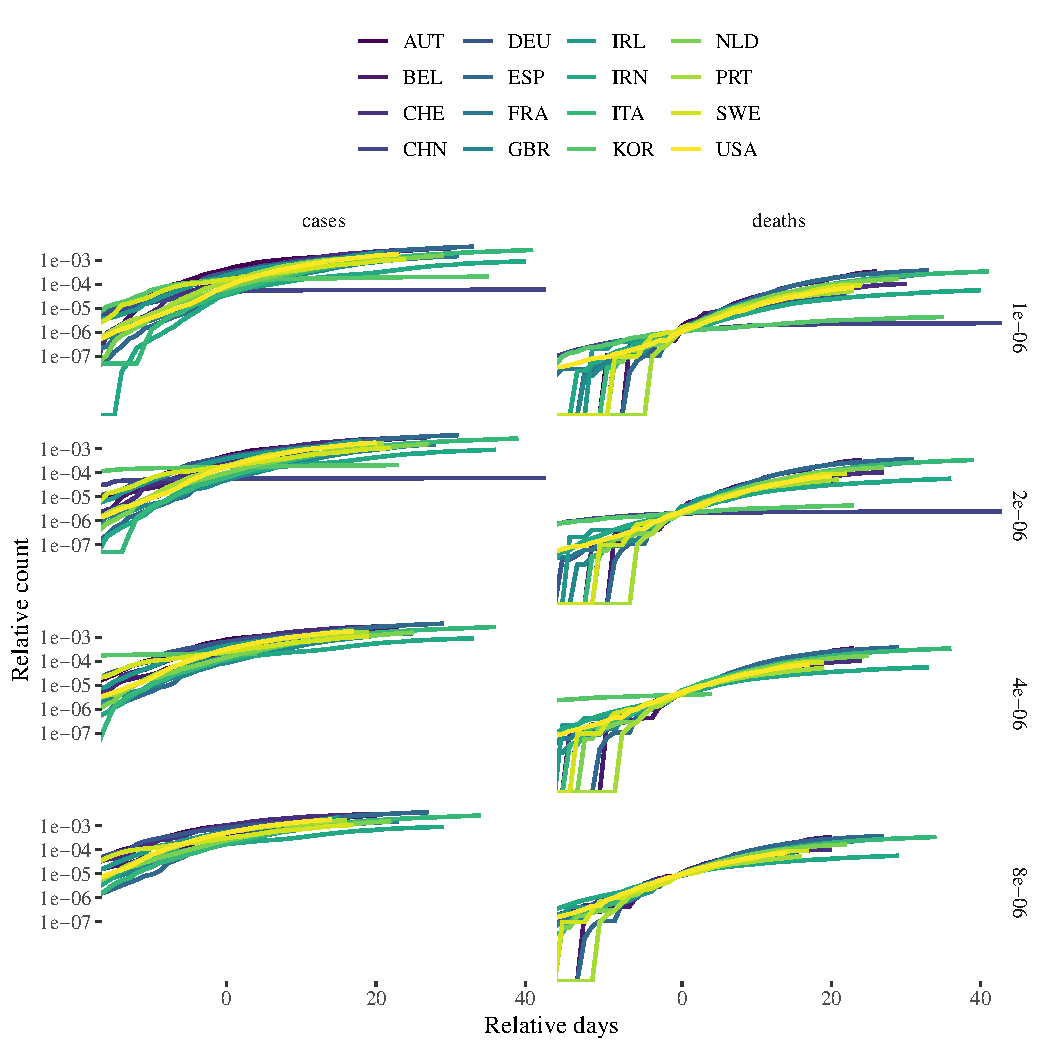
\includegraphics[width=1\textwidth]{../figs/ecdc_align_all.pdf}
  \caption{\label{fig:aligned_data} Relative case and death counts of
    selected countries. Dates are aligned relative to the first day
    that relative death counts exceed one (top) or ten (bottom) per
    million respectively.}
\end{figure}

Here, I do not attempt to explain all these country specific
differences. Instead, the relation between relative death and case
counts is considered. While relative death counts exhibit similar time
courses the corresponding relative case counts $d_t$ are more variable
when aligned in the same fashion, i.e. relative to the first day that
$d_t$ exceeds a given threshold. As I will argue now, most of this
variability can be explained with two readily interpretable
parameters.

\begin{hypothesis}
  \label{hyp:delay}
  There is a well defined country specific delay between reported
  cases and deaths.
\end{hypothesis}

\fig{aligned_data} suggests that relative case counts are not aligned
as some countries, e.g. Germany, systematically lead the counts
reported in other countries, e.g. Italy. Such a difference could mean
that individuals which eventually die are admitted to longer
treatments since they had been tested positive. It could also just
reflect reporting delays due to bureaucratic reasons. In any case, it
is clearly the case that individuals die some days after they had been
tested positive.

\subsection{Case fatality rate}

This delay also needs to be taken into account when estimating the
case fatality rate (CFR). Commonly the CFR is defined as $\mathrm{cfr}
= \frac{d_t}{c_t}$. Not surprisingly this estimate is highly variable
and changes systematically over time, especially at the beginning of
an epidemic. Instead, taking into account that individuals that had
been tested positive will not die on the same day but after some delay
$\tau$ (if at all), I define
\begin{align}
  \label{eq:cfr}
  \mathrm{cfr}_{\tau} &= \frac{d_t}{c_{t - \tau}} \; ,
\end{align}
i.e. comparing current death with previous case counts.

\begin{figure}
  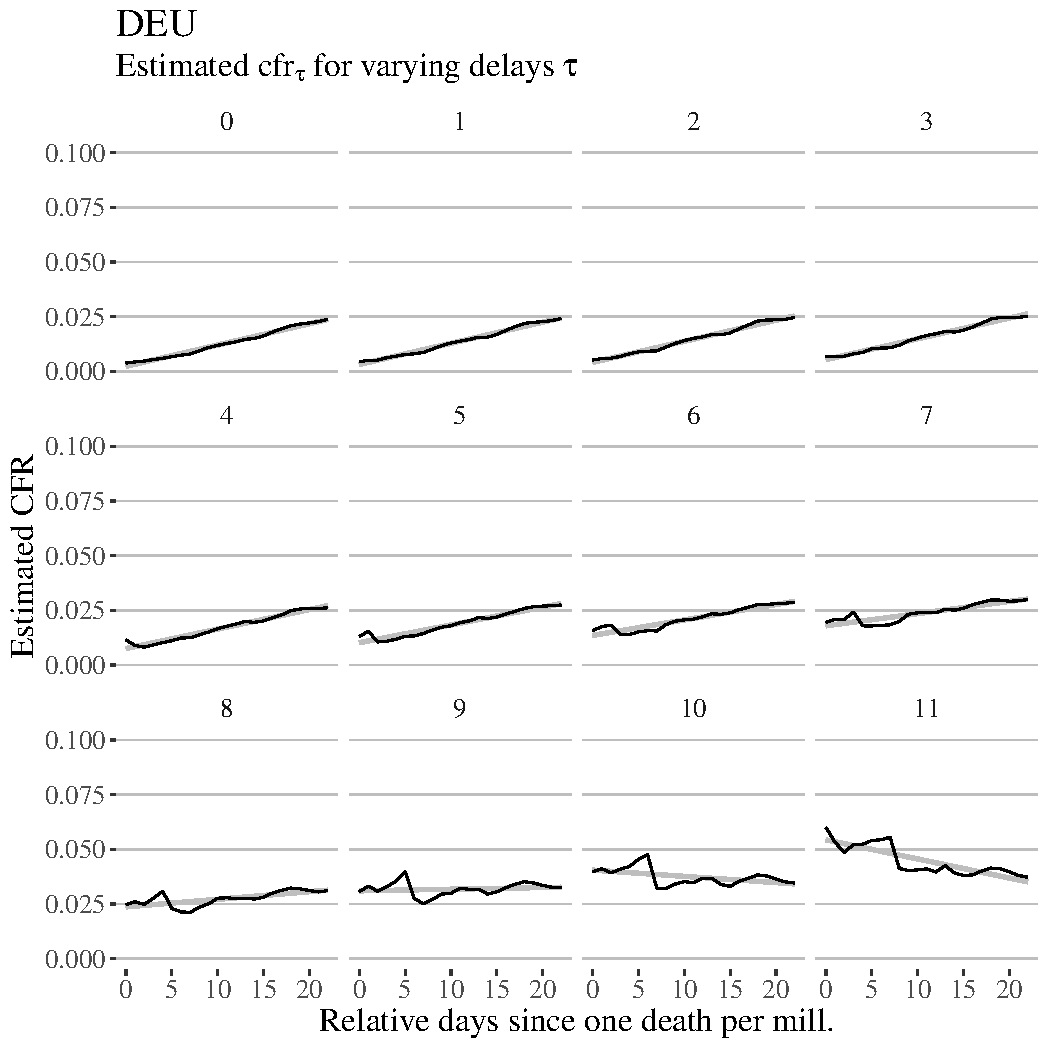
\includegraphics[width=0.495\textwidth]{../figs/ecdc_cfr_delay_DEU.pdf}
  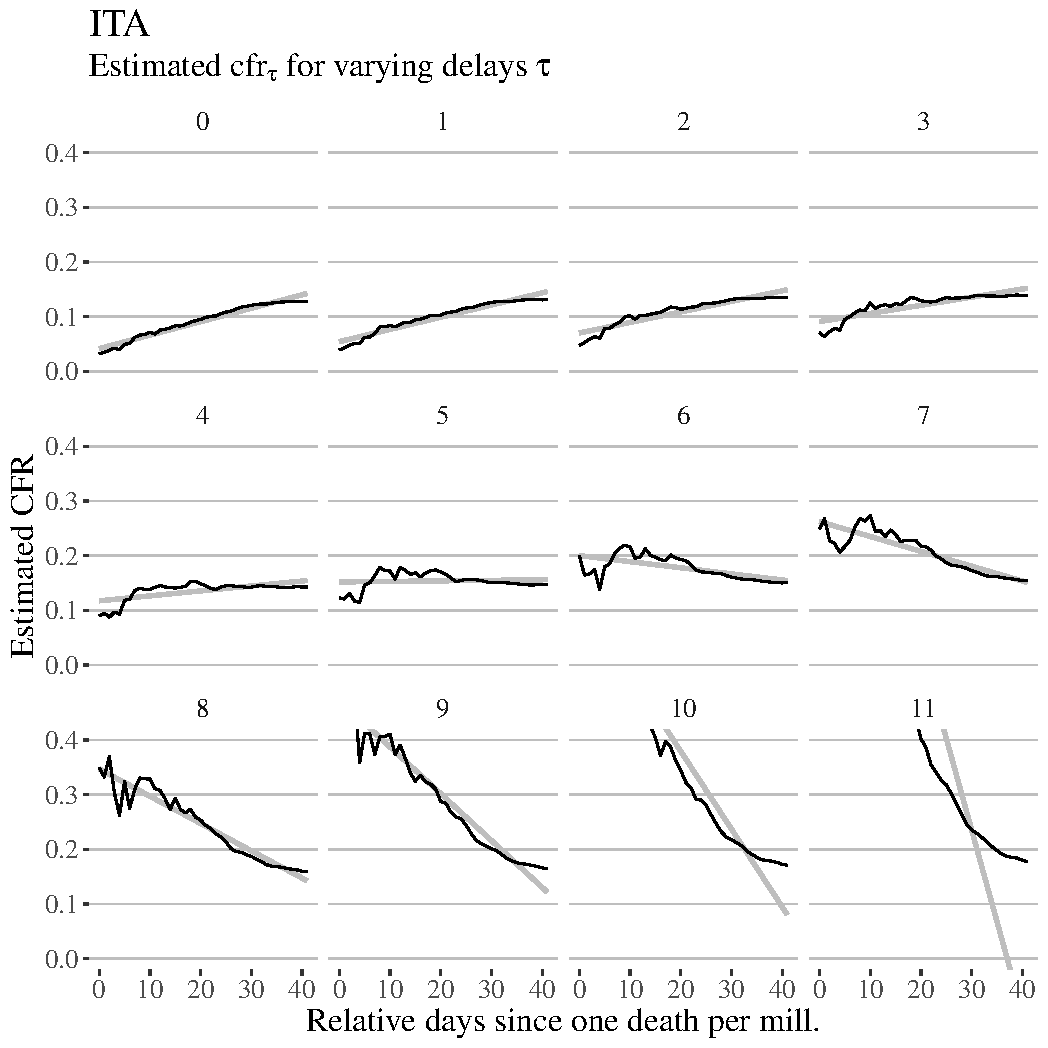
\includegraphics[width=0.495\textwidth]{../figs/ecdc_cfr_delay_ITA.pdf}
  \caption{\label{fig:cfr}}
\end{figure}
\fig{cfr} shows the CFRs estimated for Germany and Italy in this
fashion, i.e. for different delays $\tau$. The estimate using $\tau =
0$ rises over time simply reflecting that the death counts only later
catch up with the exponentially growing case counts. Interestingly,
for each country there exists as characteristic delay at which the
estimated CFRs are essentially constant. Thus, reflecting the
hypothesized delay between reported cases and deaths.

\begin{hypothesis}
  \label{hyp:cfr}
  The true case fatality rate is the same for all countries.
\end{hypothesis}



\bibliographystyle{abbrv}
\bibliography{notes}

\clearpage

\appendix

\section{Additional figures}

\begin{figure}
  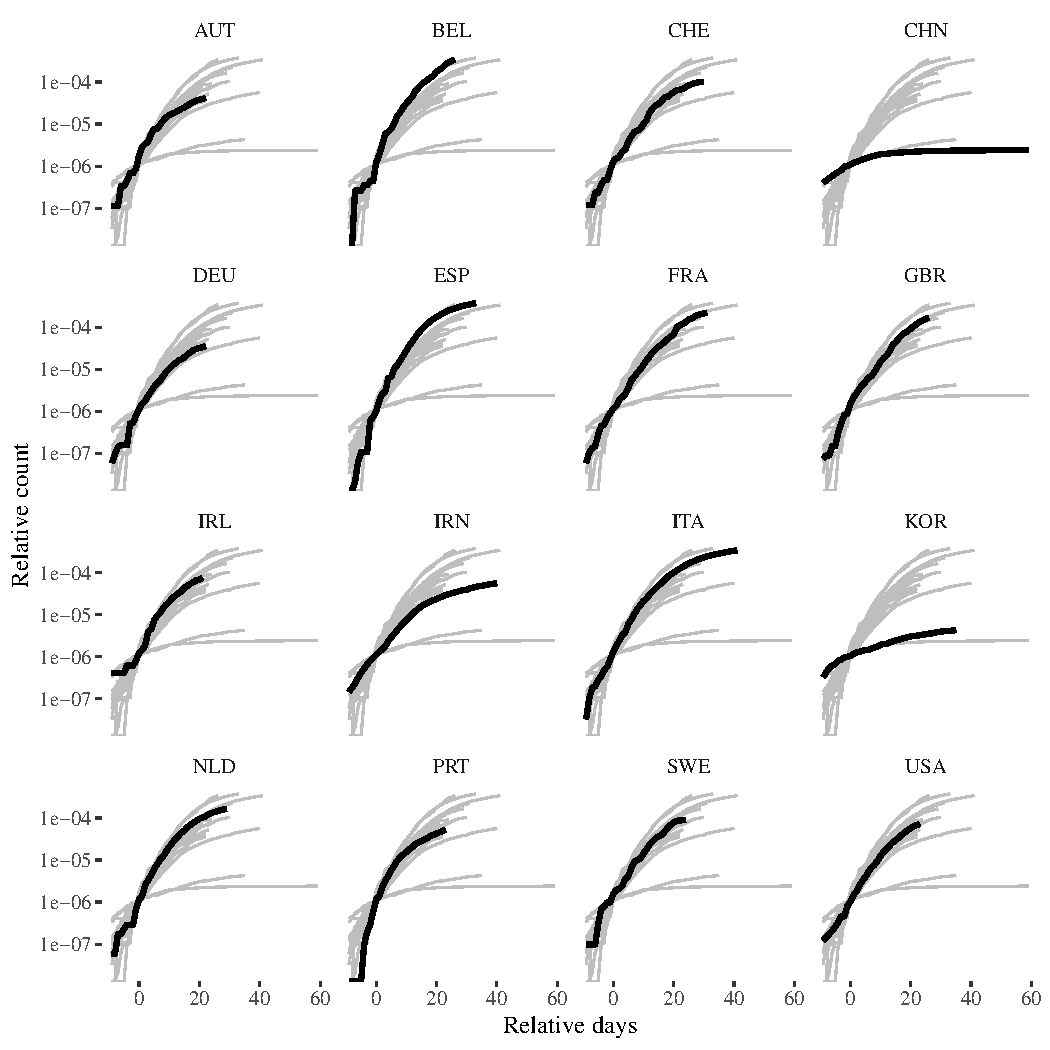
\includegraphics[width=1\textwidth]{../figs/ecdc_aligned_onepermill_nyt.pdf}
  \caption{\label{fig:align_nyt}}
\end{figure}

\end{document}
